\documentclass[tikz]{standalone}

\usepackage{chemformula} % used for \ch and \text

\usetikzlibrary{positioning, calc, decorations.pathreplacing}

\begin{document}
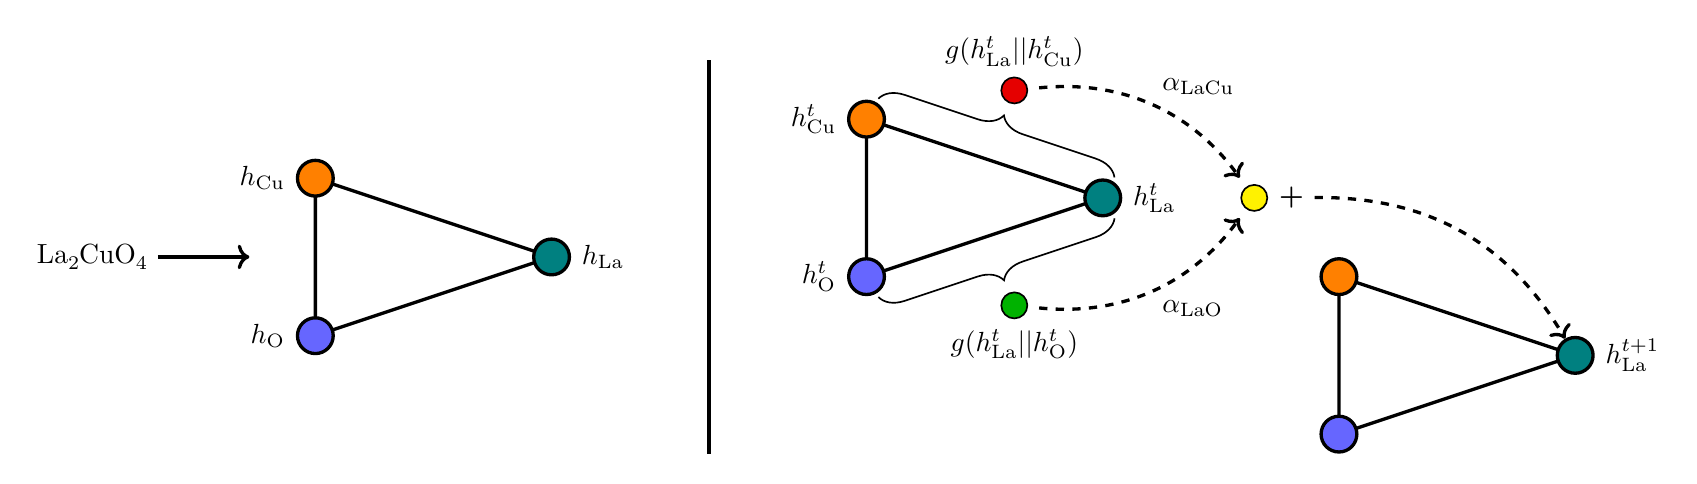
\begin{tikzpicture}[very thick, vertex/.style={draw, circle, minimum size=3ex}]

  \draw (0,0) coordinate[vertex, fill=teal, label=right:$h_\text{La}$] (h_La) -- ++(-3,-1) coordinate[vertex, fill=blue!60, label=left:$h_\text{O}$] (h_O) -- ++(0,2) coordinate[vertex, fill=orange, label=left:$h_\text{Cu}$] (h_Cu) -- cycle;

  \node[left=2cm] at ($(h_O)!0.5!(h_Cu)$) (La2CuO4) {\ch{La2CuO4}};
  \draw[->] (La2CuO4) -- ++(2cm,0);

  \draw[ultra thick] (2,-2.5) -- (2,2.5);

  \begin{scope}[shift={(7,0.75)}]
    \draw (0,0) coordinate[vertex, fill=teal, label=right:$h_\text{La}^t$] (h_La_t) -- ++(-3,-1) coordinate[vertex, fill=blue!60, label=left:$h_\text{O}^t$] (h_O_t) -- ++(0,2) coordinate[vertex, fill=orange, label=left:$h_\text{Cu}^t$] (h_Cu_t) -- cycle;

    \draw (6,-2) coordinate[vertex, fill=teal, label=right:$h_\text{La}^{t+1}$] (h_La_tp1) -- ++(-3,-1) coordinate[vertex, fill=blue!60] (h_O_tp1) -- ++(0,2) coordinate[vertex, fill=orange] (h_Cu_tp1) -- cycle;

    \draw[semithick, decorate, decoration={brace, amplitude=2ex}] ($(h_La_t)-(120:0.3)$) -- ($(h_O_t)-(120:0.3)$) coordinate [vertex, minimum size=2ex, fill=green!70!black, midway, shift={(1.5ex,-4ex)}, label=below:$g(h_\text{La}^t || h_\text{O}^t)$] (g_La_Cu);
    \draw[semithick, decorate, decoration={brace, amplitude=2ex}] ($(h_Cu_t)+(60:0.3)$) -- ($(h_La_t)+(60:0.3)$) coordinate [vertex, minimum size=2ex, fill=red!90!black, midway, shift={(1.5ex,4ex)}, label=above:$g(h_\text{La}^t || h_\text{Cu}^t)$] (g_La_O);

    \coordinate[semithick, vertex, minimum size=2ex, fill=yellow, right=1.5 of h_La_t] (alpha);
    \draw[dashed, ->, shorten <=4, shorten >=4] (g_La_O) edge[bend left] node[midway, above right] {$\alpha_\text{LaCu}$} (alpha);
    \draw[dashed, ->, shorten <=4, shorten >=4] (g_La_Cu) edge[bend right] node[midway, below right] {$\alpha_\text{LaO}$} (alpha);

    \node[right=0 of alpha] (plus) {\textbf +};
    \draw[->, dashed] (plus) edge[bend left] (h_La_tp1);
  \end{scope}

\end{tikzpicture}
\end{document}
